
\documentclass{article}
\usepackage{hyperref}

\usepackage{graphicx}

\title{Fiberassign performance}
\author{Jaime E. Forero-Romero \footnote{{\texttt{j.e.forero.romero@gmail.com}}}\\Universidad de los Andes}
\date{\today}

\begin{document}
\maketitle
\begin{abstract}
In this document I use DR7 data to show that fiberassign
meets the desired performance in terms of total fiber usage and number
of calibration targets.  
\end{abstract}

\section{Introduction}
{\texttt fiberassign} is the software that computes the assignment of
fibers to DESI targets. 

The following are the minimal requirements on its performance
\begin{itemize}
\item Fiber assignment uses required fraction of fibers IN.DAT-7002
\item Fiber assignment provides sufficient calibration fibers IN.DAT-7003
\end{itemize}

In this document I present the results of running {\texttt
  fiberassign} on targets from DR7 to demonstrate how the two
requirements mentioned above are met. 
Furthermore I list some computational performance results to
understand how long does it take to run the code and how many
resources does it use.

\section{Software and input data}

For this report I use tag {\texttt 0.10.1} of {\texttt fiberassign}. 

The input targetting data comes from DR7. On NERSC the files can be found here:
{\texttt{/project/projectdirs/desi/target/catalogs/dr7.1/PR372/}}

The targeting files need to be prepared in order to pass them to
fiberassign.
The code that prepares the data and runs fiberassign can be found
here:
\url{https://github.com/forero/fiberassign_explore/blob/master/py/fiberassign_on_DR7.py}.
The script needs to be executed as {\texttt{python fiberassign\_on\_DR7.py --program dark
--size large}} to produce the outputs analized in this report.

The most important features to highlight about fiberassign are the
following:

\begin{itemize}
\item It receives as input three files: a list of science targets, a
  list of good sky locations and a list of standard
  stars. 
\item The code fills up to 400 sky fibers and 100 std fibers if the
  number density of those calibration targets is high enough.
\item Afterwards the code proceeds to assign science targets.
\item If there are unused fibers after the science assignment process
  those fibers are filled with sky targets if available.
\item There are also BADSKY locations that are treated as another
  science target with the lowest priority.
\end{itemize}



We only use targets that can be observed in dark time. 
With this restriction we end up with 7054 DESI tiles that correspond
to dark time and overlap with the DR7.1 footprint. 
This selection returns 36M targets, 1.3M standard stars and
22M sky locations.
Furthermore, we restrict our analysis on tiles that have complete imaging
within $128<$RA$<225$128 and $-7<$dec$<32$.  This selection reduces
the total number of tiles to 2510. 

\section{Results}

Figure \ref{fig:used_fibers} summarizes the results, it shows the
histograms of the number of used fibers per tile.
The label shows the average and the standard deviation computed over
the tiles. 

These histograms show that all tiles use at least 4996 fibers; 
on average $99.98\%$ of the fibers are used.
1817 tiles out of the 2510 ($72\%$) use all 500 fibers.
All tiles have at least 400 SKY locations and all tiles have 100 STD
fibers, except one with 99 STD fibers. 

\section{Performance}
Runnig fiberassign on a cori login node takes 2 hours and  uses a
peak of 38GB of RAM.
The wallclock time is proportional to the number
of tiles. In this case we have that the code assigns on average one
tile per second. 


\begin{figure}[!h]
\begin{center}
\begin{center}
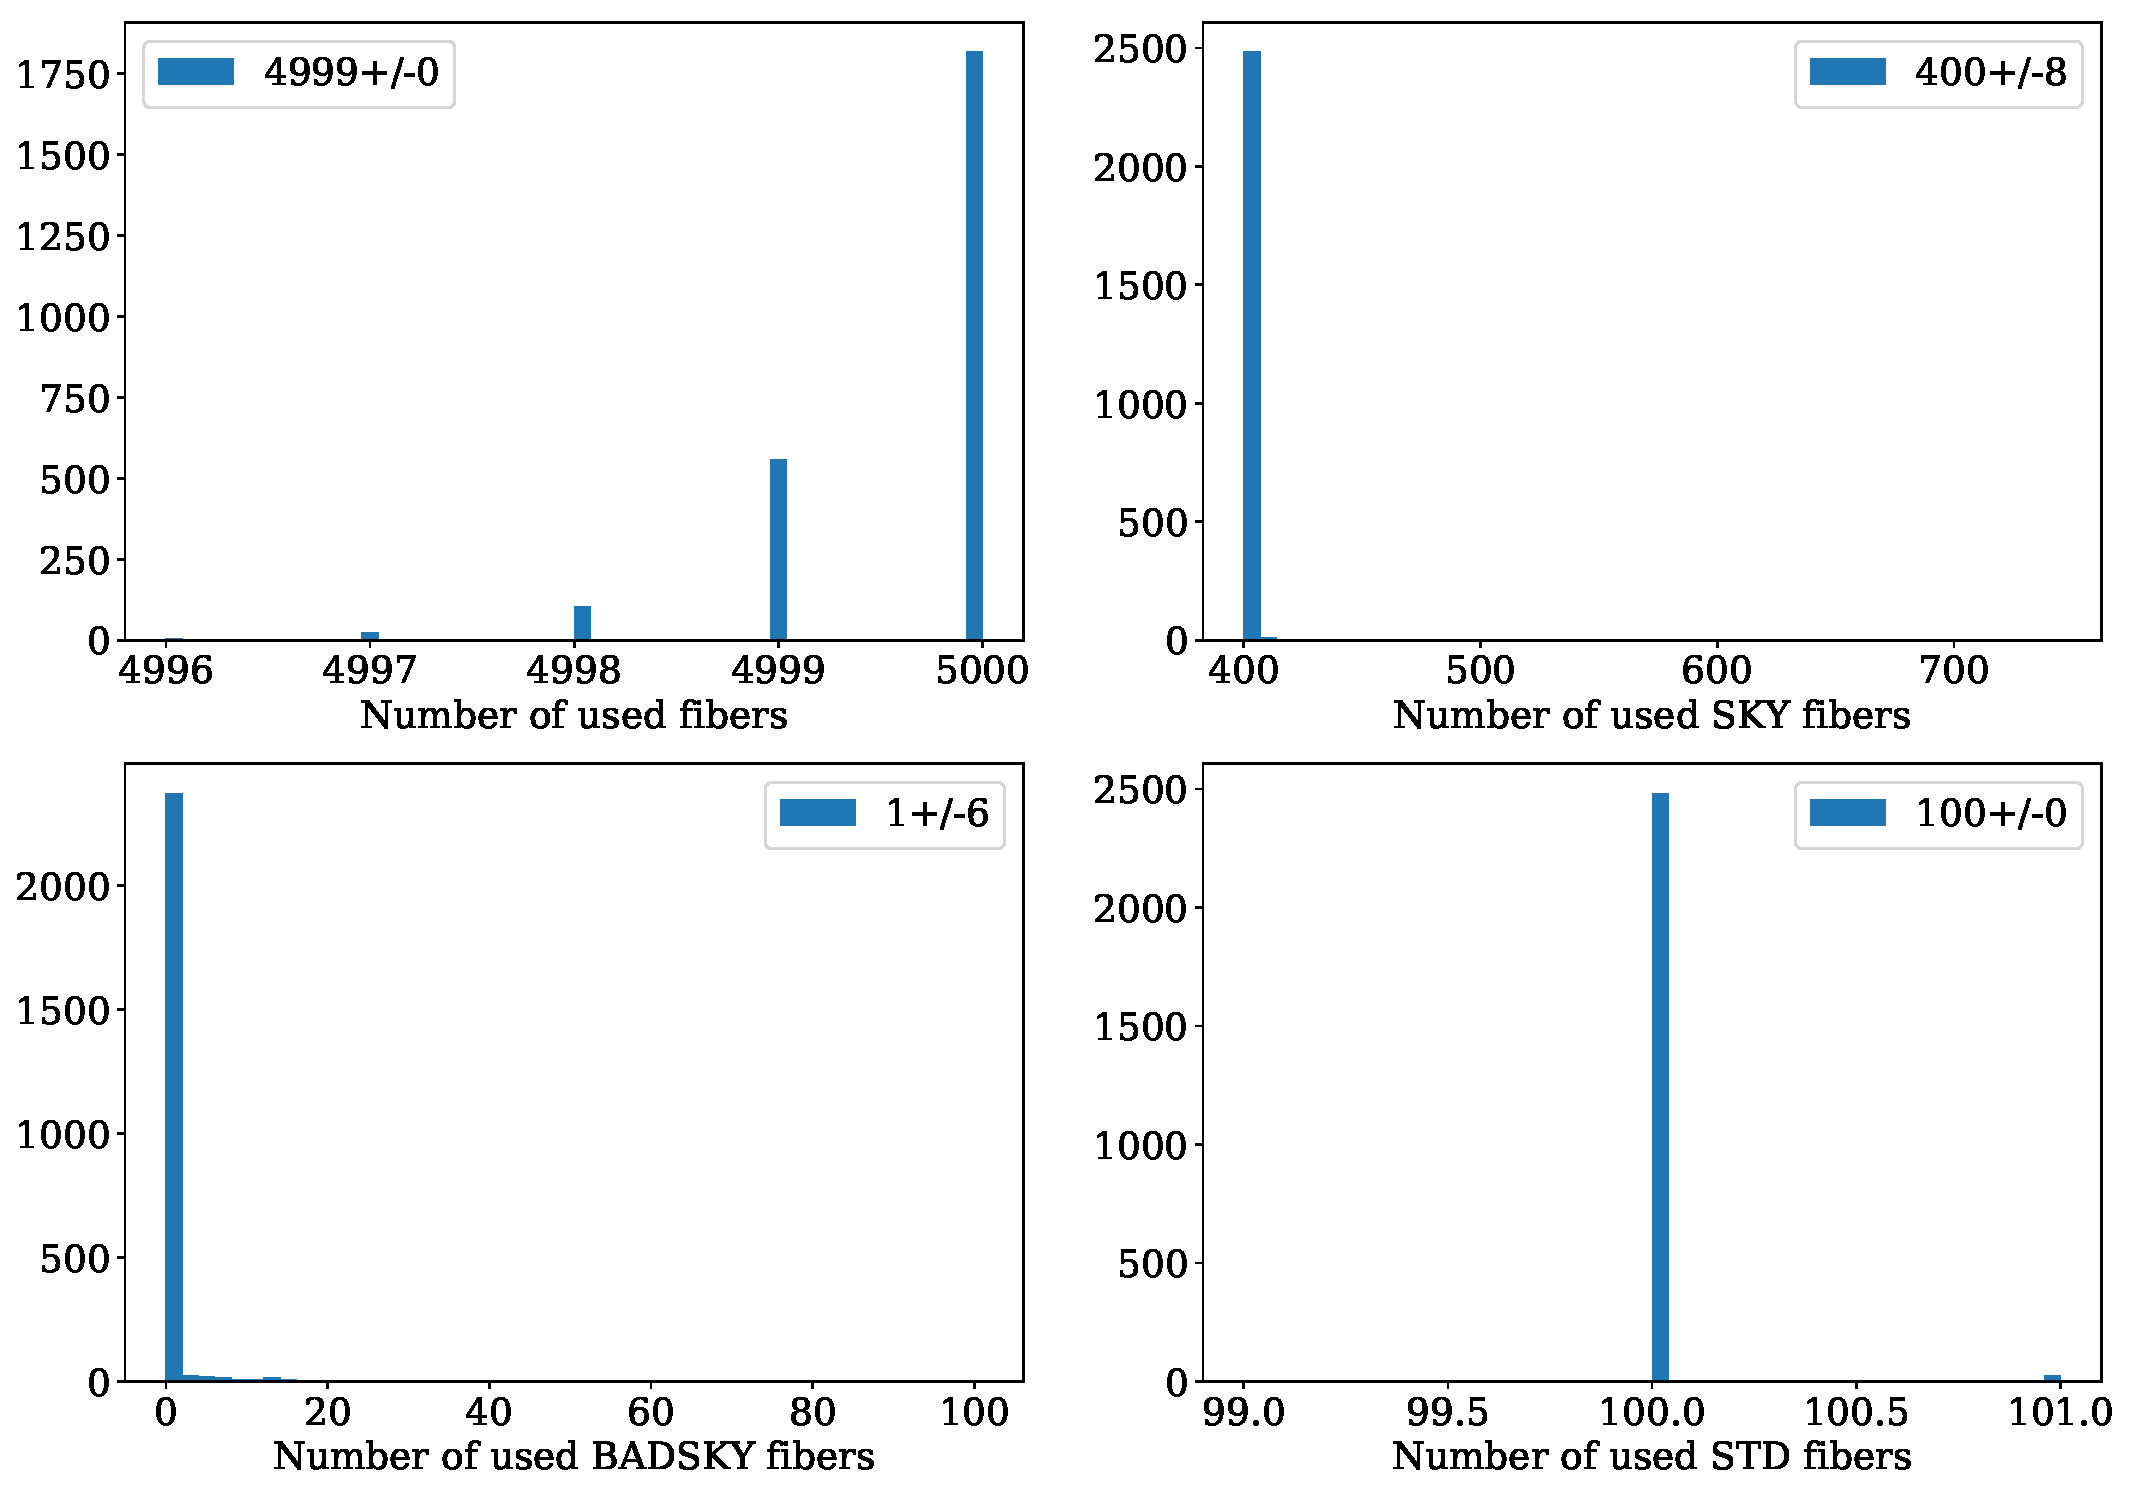
\includegraphics[scale=0.40]{used_fibers.pdf}
\end{center}
\caption{
Histograms with the number of total assigned fibers, SKY fibers, 
BADSKY fibers and STD fibers.
\label{fig:used_fibers}}
\end{center}
\end{figure}


\end{document}

\begin{itemize}
\item SKY: fibers for sky calibration.
\item STD: fibers on standard stars.
\item BADSKY: fibers on BADSKY locations

\item SCIENCE: fibers on science targets.
\end{itemize}


The label shows the average and the standard deviation computed over
the tiles. 
This Figure shows that on average $99.92\%$ of the fibers are used,
on average $397$ are used for sky locations and $99$ are used for
standard stars. 
On average $4499$ science targets are observed per tile.
The small fluctuations in the number of sky location and standard star fibers
is due to changes in the input number densities for those targets. 
The input sky and stdstar catalogs must be tuned to have everywhere
the desired number of targets per tile. 

Figure \ref{fig:used_ra_dec} demonstrates that fiber assignement uses
the required fraction of fibers and provides sufficient calibration
targets. 


